\setcounter{footnote}{0}
\setcounter{section}{0}
\setcounter{ExNo}{0}
\begin{center}
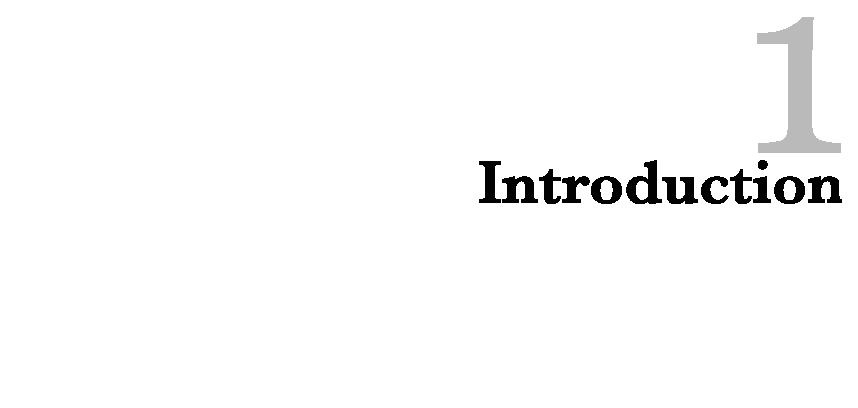
\includegraphics{chapter1.eps}
\end{center}
\section*{}
\addcontentsline{toc}{section}{\Large{Chapter 1: Introduction}}
\section{Downward movement} \label{Ch1_downward_movement_sec}
The goal of much research in generative grammar is to uncover the mechanisms underlying apparent mismatches between the purported base-generated positions of syntactic constituents and their ultimate locations in the phonological and/or semantic representations. Determining what motivates---and what limits---these transformations of linguistic structure is thus one of the primary concerns of such investigation. In this thesis, I focus on one type of transformation, namely those cases in which a morpheme is pronounced in a position that is arguably lower than its base-generated position. In all of these cases, a morpheme has adjoined to or within a word that overtly occupies a lower syntactic position than the first merger site of that morpheme in the derivation, indicating that the morpheme has undergone a downward movement.

The sort of transformation that we will be addressing has posed a perennial challenge for most generative models of syntactic derivation, which limit transformational operations to upward movement, disallowing movement to positions lower in the syntactic structure. Given the undeniably apparent cross-linguistic scarcity of structural transformations that appear to be downward, it has been posited that such movements are precluded by fundamental properties of syntactic computation. For example, it was proposed under Government and Binding Theory (GB) \citep{chomsky1981} that any trace of a syntactic object must be antecedent-governed (i.e.\ locally c-commanded) by that syntactic object. Under this view, traces, like anaphors, are variables that must be properly bound.\footnote{We will investigate this claim further in Chapter 3, where I suggest that, in cases of head movement, this condition is obviated as a result of total syntactic reconstruction at LF.} Thus, a syntactic structure that exhibits downward movement, effectively creating an unbound trace, would be deemed illicit. Any apparent downward transformation was instead argued to take place on the PF branch, surfacing as the result of some filter on phonological representations (e.g.\ \posscitet{chomsky1981} Rule R), thus allowing for the total absence of downward movement in syntactic computation. The Minimalist Program (MP) \citep{chomsky1995} continues this tradition of upward-only movement in the syntax. Indeed, under MP, most, if not all, cases of apparent downward movement, such as affix-hopping, are argued to be illusory, and instead arise from the combination of a lexicalist morphology and upward covert movement.\footnote{Under this view, all morphologically complex words are formed before they enter the syntactic derivation, and so they may be pronounced in a low position in their full morpho-phonological forms before undergoing covert movement to higher heads. We will discuss this model further in later sections.}$^{,}$\footnote{Note also that, within MP, movement operations have been argued to be constrained by the Extension Condition, which requires that all structure-building operations occur cyclicall�y, targeting only the topmost node of the syntactic derivation (i.e.\ the root node) as the site of merger and re-merger of syntactic elements (\citenop{chomsky1993}, \citenop{epstein_etal1998}, \citenop{zhang2004}, among others). However, head movement in general is problematic under the Extension Condition, since head-adjunction does not target the root node (but see \citet{matushansky2006} for an attempt to reconcile head movement with the Extension Condition). Furthermore, even phrasal movement is argued to often violate (a strict version of) the Extension Condition (e.g.\ \posscitet{richards2001} ``tucking in''). Given these independent objections to the Extension Condition, I will not consider such a condition to be an inviolable principle of syntactic derivation. For example, I will not assume that a violation of the Extension Condition in cases of head-to-head Lowering provides sufficient reason to preclude the existence of such a structural transformation. However, we will return to this issue briefly throughout this thesis (see, for example, Chapter 5, \S\ref{covert_mov}).} We thus observe that, within the most widely accepted paradigms of generative grammar, downward movements have either been relegated to a position outside of the core transformational theory, or have been claimed to be non-existent.

In this thesis, following \citet{embick_noyer2001}, I argue not only that downward movements exist, but also that they can be incorporated into the fundamental, overarching architecture of derivational processes, including both narrow syntactic and post-syntactic operations. I propose that downward movements are not theoretically exceptional, but are rather the result of inherent properties of linguistic computation, including, above all, the interface of syntax and phonology. In particular, I claim that head-to-head Lowering is driven by properties of cyclic Spell-out to the PF branch (\citenop{chomsky2001}, \citenop{svenonius2001}, \citenop{uriagereka1999}, and many others), and that even Local Dislocation (i.e.\ morphological merger in the post-Spell-out morpho-phonological representation) can play a role in certain processes previously argued to be purely syntactic, namely feature-checking. In this way, I argue that a principled account of downward movements gives us insight into certain aspects of the derivational architecture, including, but not limited to, the timing and domain of cyclic Spell-out to the interfaces. Therefore, the central goal of this thesis is to show how all types of transformational processes can be analyzed in an inclusive manner as core parts of a single derivational process, thus allowing us to develop a more complete, organic model of linguistic computation from start to finish.


\section{Architecture of the PF branch}
Note that even recent treatments of downward movements (e.g.\ \citenop{embick_noyer2001}) relegate all downward movement to the PF branch, maintaining the restriction against narrow syntactic downward transformations. We will also adopt this model of downward movement for much of this thesis, but will ultimately come to question whether it is accurate (see Chapter 3, \S2.2.3).\footnote{In particular, I will address whether head-to-head Lowering occurs in the narrow syntactic structure itself or the post-Spell-out morpho-syntactic structure found on the PF branch. Note, however, that this distinction in the locus of Lowering will not affect any analysis preceding this discussion in Chapter 3, and that I will maintain throughout this thesis that Lowering is, at least in a sense, a post-Spell-out operation; i.e.\ Lowering is driven by the interface of narrow syntax with PF.} We thus begin with an overview of the architecture of the PF branch that will be assumed throughout most of this work, using representative examples to illustrate the two types of downward transformations available to linguistic computation, namely Lowering and Local Dislocation. In the following sections, I will show that it is often difficult to pinpoint the exact transformation that is operative in a downward movement, but that it is possible to develop a set of analytical criteria that will help us to decipher which type of transformation is responsible for individual cases of apparent downward movement. However, before we begin to investigate the details of these post-Spell-out operations, we must first situate the scope of this investigation within a particular theory of morphology, as our main concern will be downward transformations that affect the structure of individual words.

\subsection{Lexicalist vs. Distributed Morphology}
Under lexicalist theories of morphology (e.g.\ \citenop{bresnan2001a}, \citenop{chomsky1995}, \citenop{disciullo_williams1987}, \citenop{jensen1990}, \citenop{lieber1992}, \citenop{pollard_sag1994}), complex words (i.e.\ words that are formed from the combination of two or more morphemes) are constructed in a pre-syntactic generative lexicon. That is, both mono- and poly-morphemic words enter into the syntax as readymade structures. In the case of verbal inflection in English, this requires that verbs enter into the syntax pre-specified for agreement and/or tense features. For example (where each element contained within the curly brackets `\{\}' represents an individual lexical item created before syntactic derivation):\footnote{Throughout this thesis I will adopt a {\it v}P-shell model of verb phrases in which the main or root verb V invariably moves to the light verb projection \textit{v} (\citenop{larson1988}, \citenop{kratzer1996}). See Chapter 2 for further discussion on the fine structure of {\it v}P.} 

\singlespacing
\begin{quote}
\begin{minipage}{5in}
\ex. \label{Iwalked_lex_tree} \textit{I walked.} 

\Tree
[.TP \qroof{\{\textit{I}\}}.DP_i 
[.TP T\\\{\sc{past}\} 
[.\textit{v}P t_i
[.\textit{v}P [.\textit{v} V_j\\\textit{\textbf{walked}}\\\mbox{\{\textit{walk}, \sc{past}\}}  \textit{v}  ] [ t_j ].VP
].\textit{v}P ].\textit{v}P ].TP ]

\end{minipage}
\end{quote}
\onehalfspacing
I follow \posscitet{chomsky1957} fairly uncontroversial claim that inflected verbs are divisible into discrete underlying syntactic objects, namely tense T (i.e.\ INFL) and the bare verb V. Note that certain narrow syntactic transformations target tense as a separate constituent from the verb; for example, T-to-C movement in English interrogatives (e.g.\ \textit{Did John leave?}). This then suggests that T at least forms a discrete syntactic node; i.e.\ T is merged as its own syntactic head, as in (\ref{Iwalked_lex_tree}).\footnote{Under a lexicalist morphology, this also suggests that the pre-syntactic generative lexicon can foresee whether T-to-C movement will eventually occur, as the morphological form of the verb that is created in an interrogative does not contain a T morpheme. Such a system requires that the lexicon create an inflected verb when the numeration contains a declarative C, but create an uninflected verb when the numeration contains an interrogative C. Given the absolute absence of double-tensed forms like \textit{*Did John left}, it is unclear how the lexicon makes this determination, unless a look-ahead is possible, or, alternatively, several crashing structures may possibly be derived before a converging one is created.}  Moreover, since tense in English may undergo head movement to a higher position without also raising the V head, it must necessarily be merged in a position from which it c-commands the verb, as the verb clearly does not intervene between the base-generated positions of T and the higher C to which T is attracted. Otherwise, the verb would necessarily also undergo raising during T-to-C movement, due to the \textit{Head Movement Constraint} (HMC) (\citenop{travis1984}); if the verb intervened between T and C, then the HMC would require that the verb head also be ``picked up'' and carried along during T-to-C movement, contrary to fact. Given this, it cannot be the case that tense and the verb are merged solely as a complex constituent, but that tense is at least also merged as a completely separate higher element.

Accordingly, under the view of lexical morphology, tense features must be represented twice in the derivation of (\ref{Iwalked_lex_tree}); once on the pre-syntactically constructed verb and once on the head of TP. If the tense features in these two positions match, then the derivation converges, as the inflected verb may be spelled out in the position represented in (\ref{Iwalked_lex_tree}), but may raise covertly to T to check its inflectional features against those in T.\footnote{This is admittedly an oversimplification of lexicalist morphology. However, what should be noted is simply that, under this view, features relating to tense must be dispersed throughout multiple positions in the tree.} Notably, since (\ref{Iwalked_lex_tree}) is the structure that is sent to PF, this model does not require that T undergo a downward transformation to adjoin to the verb (see \S2.2), as the verb here already contains the inflectional morpheme, which can be checked against T later via covert movement. Indeed, it is this obviation of downward movement that led, in part, to the incorporation of lexicalist verbal morphology into the Minimalist Program.

In their theory of Distributed Morphology (DM), \citet{halle_marantz1993} reject the existence of a pre-syntactic generative lexicon, arguing instead that all morphologically complex words are derived in the syntactic and post-syntactic modules of the grammar, just as in the case of larger elements of linguistic structure (i.e.\ phrases and sentences).\footnote{See also \citet{harley_noyer1998} for an analysis that provides additional support to this model.} Under this view, syntactic derivation is the first step in the creation of any and all complex structures, with the possibility of certain further transformations occurring after the syntax interfaces with PF via the operation of Spell-out, to be discussed below. This model has two clear advantages over a lexicalist morphology. First, by reducing the number of generative modules, it creates a more economical system of linguistic derivation in which all elements are subject to a single set of syntactic and post-syntactic restrictions. Second, it allows us to dispense with feature redundancies like that seen in (\ref{Iwalked_lex_tree}). For example, under DM, the verb in (\ref{Iwalked_lex_tree}) enters the derivation with no pre-specified tense features, as in (\ref{Iwalked_DM_tree}).

\singlespacing
\begin{quote}
\begin{minipage}{5in}
\ex. \label{Iwalked_DM_tree} \textit{I walked.} 

\Tree
[.TP \qroof{\{\textit{I}\}}.DP_i 
[.TP T\\\{\sc{past}\} 
[.\textit{v}P t_i
[.\textit{v}P [.\textit{v} V_j\\\textit{\textbf{walk}}\\\mbox{\{\textit{walk}\}}  \textit{v}  ] [ t_j ].VP
].\textit{v}P ].\textit{v}P ].TP ]

\end{minipage}
\end{quote}
\onehalfspacing

\noindent
Here, DM offers two (general) theoretical possibilities to derive the complex morphological form \textit{walked}; either the verb may raise syntactically to the tense morpheme, or the tense morpheme may move downward to the verb post-syntactically. We will see in \S2.2 that it must be the latter case in English. What it is crucial to be aware of here, however, is that DM, by simplifying the representation of lexical items within the syntax, in turn also allows us to simplify syntactic procedures. Note that in (\ref{Iwalked_DM_tree}), since the verb lacks any tense features, there is no longer a need to covertly check any pre-syntactic inflectional features on the verb with those in T, as is necessary under a lexicalist model of morphology.\footnote{This does not rule out the possibility of covert verb movement, but rather allows for a theoretical model under which such movement may not be obligatory.} In the remainder of this thesis, I will adopt this model of DM and therefore assume that only individual morphemes may be merged into the syntactic derivation, and that, subsequently, all complex morphological forms are derived via syntactic and/or post-syntactic operations.\\

\subsection{A brief introduction to Lowering}
As mentioned above, the morphemes \{\textit{walk}\} and \{\textit{\sc{past}}\} in (\ref{Iwalked_DM_tree}) may theoretically be combined in two different ways under DM; either via a narrow syntactic raising operation or a post-syntactic downward transformation. However, as is well known, English verbs do not raise overtly out of {\it v}P, unlike verbs in languages such as French (\citenop{emonds1976}, \citenop{pollock1989}). This is illustrated by the asymmetric patterns of French (\ref{FrVmov}) and English (\ref{EnVmov}), in which the verb varies in its surface position relative to the {\it v}P-adjunct \textit{`completely'}.\footnote{Though I am purposefully not adopting a cartographic approach to syntactic structure with respect to adverb placement (\citenop{cinque1999}), the majority of adverbs used in this thesis to illustrate the relative positions of tense and the verb are all argued to occupy positions between the base-generated positions of T and \textit{v} within such cartographies. This, then, still suggests a downward transformation in tense-hopping languages. See Chapter 2, \S\ref{cinque_sec} for a closer examination of Cinque's functional hierarchy from the perspective of tense-hopping.} 

\singlespacing
\begin{quote}
\begin{minipage}{5in}
\ex. \label{FrVmov}
\ag. Jean \underline{oublie} \textbf{compl\`{e}tement} l'adresse.\label{FrVmova}\\
Jean forget.\sc{3s.pres} completely \mbox{\sc{det}}.address\\
`Jean completely forgets the address.'\\
\bg. *Jean \textbf{compl\`{e}tement} \underline{oublie} l'adresse.\label{FrVmovb}\\
Jean completely forget.\sc{3s.pres} \mbox{\sc{det}}.address\\

\ex. \label{EnVmov}
\a. *John \underline{forgets} \textbf{completely} the address. \label{EnVmova}
\b. John \textbf{completely} \underline{forgets} the address. \label{EnVmovb}\\

\end{minipage}
\end{quote}
\onehalfspacing
Due to the ordering in (\ref{EnVmovb}), a syntactic structure like that in (\ref{Johnforget_tree}) is assumed, in which the verb remains within {\it v}P.

\singlespacing
\begin{quote}
\begin{minipage}{5in}
\ex. \label{Johnforget_tree} \textit{John completely forgets the address.} 

\moveleft12pt\vbox{\small{\Tree
[.TP \qroof{\{\textit{John}\}}.DP_i 
[.TP T\\\{\sc{pres}\}  
[.\textit{v}P \qroof{\{\textit{completely}\}}.AP
[.\textit{v}P t_i
[.\textit{v}P [.\textit{v} V_j\\\{\textit{forget}\} \textit{v}  ]
[.VP t_j  \qroof{\{\textit{the address}\}}.DP 
].VP ].\textit{v}P ].\textit{v}P ].\textit{v}P ].TP ]\\}}

\end{minipage}
\end{quote}
\onehalfspacing
The question, of course, is how the tense morpheme gets realized on the verb if the verb does not move higher in the syntax than its position in \Last. Following the standard assumption that downward movements are prohibited in the narrow syntactic derivation, \citet{embick_noyer2001} argue that T is realized on the verb in English (and presumably other tense-hopping languages) as the result of post-Spell-out T-to-\textit{v} Lowering. We must here note that, under DM, syntactic terminals consist solely of bundles of morpho-syntactic features, and are devoid of phonological features----the non-generative pre-syntactic ``lexicon'' contains no phonological features, but only morpho-syntactic feature bundles. Phonological features are mapped to syntactic terminals during the post-Spell-out process of Vocabulary Insertion (VI) (i.e.\ late insertion). This VI process takes as its input a syntactic hierarchy of morpho-syntactic terminals and gives as its output a linearized string of morpho-phonological elements that carry phonological segments. Importantly, VI erases syntactic hierarchy during this conversion process. Taking into consideration that adjuncts and specifiers are transparent for syntactic head raising, Embick and Noyer argue that the transparency of the adjunct for the tense-to-verb tense-hopping transformation resulting from \Last implies that this is a type of head movement operation. As such, since Lowering is a head-to-head operation, it is necessarily sensitive to syntactic hierarchy, and must therefore occur before VI. However, since Lowering may not occur in the narrow syntax, by hypothesis, it must occur on the PF branch.\footnote{Note, again, that we will be refining the exact timing of Lowering with respect to Spell-out in Chapter 3.} Lowering is accordingly defined as follows:\footnote{See \S\ref{low_ld_diff_sec} below and Chapter 2 for the definition and importance of the `X$^{0}$' notation.} 

\singlespacing
\begin{quote}
\begin{minipage}{5in}
\ex. \textit{Lowering (to be revised)}\\
A head X$^{0}$ may be lowered to the head of its complement Y$^{0}$ after Spell-out, but before Vocabulary Insertion.
\a.[][$_{XP}$ X$^{0}$ ... [$_{YP}$ ... Y$^{0}$ ... ]] $\rightarrow$ [$_{XP}$ ... [$_{YP}$ ... [$_{Y}$\raisebox{-3pt}{$^{\circ}$} Y$^{0}$ + X$^{0}$] ... ]]\\

\end{minipage}
\end{quote}
\onehalfspacing
Under this analysis, tense-hopping is blocked when T does not take {\it v}P as a complement at Spell-out (e.g.\ in cases of an intervening NegP projection, T-to-C movement, etc.). In Chapter 3, we will see evidence that gives us reason to reject the Lowering analysis of English tense-hopping, such as comparative data from {\it v}P-movement in English and Swedish, another tense-hopping language; rather, English tense-hopping is argued to result from morpho-phonological merger on the PF branch, i.e.\ Local Dislocation. However, in Chapter 2, we will also see evidence of Lowering in other languages that allows us to maintain the definition in \Last, with one or two important modifications.

We must note that, while the definition in \Last might adequately explain the structural properties of Lowering, it gives no indication as to why Lowering occurs. Indeed, previous studies of Lowering have not addressed the issue of the motivations underlying these operations. Though much attention has been paid to the reasons behind upward head and phrasal movement in linguistic theory, there has been no explanatory theory developed to account for why head-lowering occurs, and therefore how it might fit into an overall model of structural transformations. One of the primary goals of this thesis is to develop such a theoretical model, under which the different patterns of Lowering and Raising are accounted for via principled means. In particular, I argue that Lowering, like all other transformations of syntactic structure, is feature-driven, and that, contra previous theories of the relationship between feature-checking and Spell-out, which limit feature-checking to the pre-Spell-out, narrow syntactic derivation, Lowering checks uninterpretable features after (or rather during) Spell-out of the narrow syntax. This suggests that the pre-Spell-out narrow syntactic derivation is not the only domain in which morpho-syntactic feature-checking may occur. As I will argue, Lowering simply occurs when narrow syntactic feature-checking via raising is impossible, due to the effects of cyclic Spell-out.

To explain a bit further, note that Lowering, as it necessarily occurs before VI, cannot be sensitive to phonological concerns (e.g.\ word minimality, prosody, segmental information, etc.), but must rather be driven by concerns of the morpho-syntax. Assuming that all structural transformations of morpho-syntactic elements are driven by the checking requirements of uninterpretable features, head-to-head Lowering should be no exception. Thus, Lowering must be feature-driven. However, transformations to satisfy the requirements of uninterpretable morpho-syntactic features are not generally considered to fall within the domain of post-Spell-out operations, but are rather thought to occur in the narrow syntactic derivation before Spell-out, or, in the case of weak features, LF syntax. In fact, it has been argued (e.g.\ \citenop{svenonius2004}) that all strong uninterpretable formal features must be checked before Spell-out to PF. However, Lowering is a post-Spell-out operation that must necessarily occur as the result of a feature-checking requirement. Taking this into consideration, it must be the case that feature-checking can occur after Spell-out.\footnote{Or, as I argue in Chapter 3, after a phase has been triggered for Spell-out.} I return to this issue in subsequent chapters and argue that, in fact, feature-checking after Spell-out is not only possible, but is also a conceptual necessity under the Minimalist Program \citep{chomsky1995}. In particular, I postulate a Strong Minimalist Feature-checking Hypothesis (SMFH), under which feature-checking may take place very late in the overall derivation. I claim that, given that post-Spell-out operations (e.g.\ Lowering and Local Dislocation) take place before the representation is evaluated at the actual articulatory-perceptual (i.e.\ pronunciation) interface, and that strong uninterpretable features must simply be checked before this interface is reached, this necessarily allows for features to be checked after Spell-out, but before the representation interfaces with the A-P system; that is, within the domain of post-Spell-out transformations on the PF branch. In Chapters 3 and 4, I develop of a model of Spell-out that allows for this conceptually desirable scenario.

For now, we have seen that Lowering is argued (e.g.\ by \citeauthor{embick_noyer2001}) to be a post-Spell-out downward head-to-head movement occurring on the PF branch before VI. Let us now turn to transformations after VI.

\subsection{A brief introduction to Local Dislocation}
There are certain downward transformations that cannot be derived via Lowering, as defined in \Last. Consider the following canonical example of the superlative transformation in English (note that this general pattern also holds for the comparative construction in English with \textit{-er/more}):

\singlespacing
\begin{quote}
\begin{minipage}{5in}
\ex. \label{super_sent_ex}
\a. She is the smart-est student. \label{super_sent_exa}
\b. *She is the intelligent-est student. \label{super_sent_exb}
\c. She is the mo-st intelligent student. \label{super_sent_exc}

\end{minipage}
\end{quote}
\onehalfspacing
\citet{abney1987} argues that it is the structure in (\ref{super_sent_exc}) that most closely mirrors the underlying syntactic/semantic structure of the superlative construction, giving us a pre-Spell-out syntactic structure like the following for the example in (\ref{super_sent_exa}), where the superlative degree operator takes syntactic and semantic scope over the AP:

\singlespacing
\begin{quote}
\begin{minipage}{5in}
\ex. \label{smartest_tree} \textit{smartest}

\Tree
[.DegP Deg\\\{\textit{-est}\} [ A\\\{\textit{smart}\} ].AP ]

\end{minipage}
\end{quote}
\onehalfspacing

The example in (\ref{smartest_tree}) could easily be accounted for under a Lowering analysis by moving the degree head to the adjective head after Spell-out. Indeed, given just the structure in (\ref{smartest_tree}), we might also account for this transformation by simply arguing that the adjective undergoes head raising in the narrow syntax to the degree head. However, in either case, we would then be unable to rule out the ungrammatical example in (\ref{super_sent_exb}). Note that the superlative transformation in English is sensitive to the phonological size of the targeted adjective. As shown in (\ref{super_list_ex}), the superlative morpheme may only undergo affixation to an adjective that is parsed into a maximum of two syllables.\\

\singlespacing
\begin{quote}
\begin{minipage}{5in}
\q\lb{super_list_ex}{\textit{Superlative constructions}}

\begin{tabular}{lllll}
~~~~~~~~~~~a. & prettiest & ~~~~~~ & e. & *beautifulest\\
~~~~~~~~~~~b. & poorest & ~~~~~~ & f. & *impoverishedest\\
~~~~~~~~~~~c. & manliest & ~~~~~~ & g. & *masculinest\\
~~~~~~~~~~~d. & drunkest & ~~~~~~ & h. & *intoxicatedest\\
\end{tabular}\\\\
\end{minipage}
\end{quote}
\onehalfspacing
The ungrammatical examples in \rf[e-h]{super_list_ex} and (\ref{super_sent_exb}) are ruled out due to the fact that the adjectives in these examples are all parsed into more than two syllables. As syllabic structure is determined based on the phonological segments of a word, phonological features must therefore be visible to the computational component when the superlative transformation is evaluated. Recall that phonological features are unavailable to the narrow syntactic derivation under DM, effectively ruling out a narrow syntactic head raising analysis of this transformation. Additionally, as Lowering necessarily occurs before phonological features have been mapped to syntactic terminals via VI, a Lowering analysis is likewise untenable.\footnote{Note that this could also be explained as optional syntactic movement. That is, either a raising or lowering operation combines the two morphemes and then, at a later stage of morpho-phonological evaluation, the structure converges only if the adjective that has participated in the head movement is mapped to two or fewer syllables, and crashes otherwise. However, unless there is first rigorous effort exerted to find an alternative, principled solution, I will reject any such analysis of purely optional transformations throughout this thesis.}  \citet{embick_noyer2001} propose that this is rather a case of the post-VI transformation Local Dislocation, in which two string-adjacent morpho-phonological elements in a linearized string are fused into a single, complex structure. Local Dislocation is defined as follows:\footnote{The notation ``Y+X'' indicates that the element X has adjoined to the element Y. For more on the nature of this morpho-phonological adjunction under Local Dislocation, see Chapter 4.}

\singlespacing
\begin{quote}
\begin{minipage}{5in}
\ex. \textit{Local Dislocation} \label{LD_def}\\
After Vocabulary Insertion, an element may adjoin to a string-adjacent element, and only to a string-adjacent element. (`$^{\wedge}$' indicates a relationship of linear precedence and adjacency in the phonological string).\\ 
\a.[][X $^{\wedge}$ Y $^{\wedge}$ Z] $\rightarrow$ [Y+X $^{\wedge}$ Z]
\b.[][X $^{\wedge}$ Y $^{\wedge}$ Z] $\not\rightarrow$ [Y $^{\wedge}$ Z+X]\\

\end{minipage}
\end{quote}
\onehalfspacing
Local Dislocation is therefore characterized as affixation under PF-adjacency, similar to previous theories of post-syntactic morphological merger (e.g.\ \citenop{bobaljik1995}).\footnote{While Local Dislocation is technically a rightward transformation in the phonological string under this definition, I will continue to refer to it as a downward transformation, given that the displacement most often involves movement of an element to another element that it c-commanded in the narrow syntactic structure (though not always; e.g.\ in right-headed languages, a morpheme X may undergo Local Dislocation with a morpheme Y that is to its right, where Y c-commanded X in the narrow syntax; see Chapter 2 \S2.3). However, it should be noted that Local Dislocation is not limited in terms of directionality, but is rather dependent solely on string-adjacency. For example, given a simple string [X $^{\wedge}$ Y], X could undergo Local Dislocation to adjoin to Y, or Y could do so to X, irrespective of c-command relations. These are both \textit{prima facie} theoretical possibilities}  In this way, if the superlative morpheme is string-adjacent to an adjective with two or fewer syllables after VI, it will undergo Local Dislocation with that adjective and will be realized as a suffix in the resulting phonological surface representation. If this condition is not satisfied, it will be realized as the phonological form \textit{most} and not undergo a merger operation (see below).

Furthermore, as Local Dislocation occurs after VI has stripped away syntactic hierarchy, intervening adjuncts are predicted to be opaque for Local Dislocation operations. This prediction is borne out.\footnote{The current argumentation follows that of \citet{embick_noyer2001}, who claim that Local Dislocation is prevented in \Next[b] due to the intervening adjunct, as in \NNext. While this is essentially correct, note that in Chapter 4 we will investigate the more intricate structure of such phrases, showing, for example, that a structure like [\textit{incredibly $^{\wedge}$ -st $^{\wedge}$ smart}] is underivable due to semantic restrictions.}

\singlespacing
\begin{quote}
\ex. \label{super_adjunct_block}
\a. * She is the incredibly smart-est student. \label{super_adjunct_blocka}
\b. She is the mo-st incredibly smart student. \label{super_adjunct_blockb}

\end{quote}
\onehalfspacing
In (\ref{super_adjunct_block}), though the adjective \textit{smart} is an appropriate target for Local Dislocation of the superlative morpheme, in terms of its size, its position in the phonological string after VI does not satisfy the criterion of string-adjacency. In (\ref{super_adjunct_block_schema}), we see that the superlative morpheme is string-adjacent to the adjunct \textit{incredibly} rather than the adjective \textit{smart}.

\singlespacing
\begin{quote}
\ex. \label{super_adjunct_block_schema} [-st $^{\wedge}$ incredibly $^{\wedge}$ smart] $\not\rightarrow$ [incredibly $^{\wedge}$ smart+-st]

\end{quote}
\onehalfspacing
Since Local Dislocation is blocked in this case, as the superlative morpheme may not skip over the intervening adjunct, I assume that the phonological component inserts the segments \textit{mo-} in order to obviate a violation of the stray-affix filter.\footnote{This might instead be a case of simple allomorphy in which the morpho-syntactic feature bundle corresponding to the superlative is mapped the phonological features /st/ when affixation under Local Dislocation is possible and the phonological features /most/ when it is not. The result would be the same. See Chapter 4 for a more detailed analysis of the superlative/comparative transformation, including satisfaction of the stray affix filter after VI, as well as a discussion of the possible category-sensitivity of Local Dislocation operations.} 

We are now left with the following order of operations after syntactic computation:\footnote{\citet{halle_marantz1993} use the term ``Morphological Structure'' to refer to the `space' between Spell-out and PF. For all intents and purposes, we will take ``Morphological Structure'' to be synonymous with ``the syntax-phonology interface.'' That is to say, the morphological operations of Lowering, Vocabulary Insertion, and Local Dislocation all occur during the point at which syntax interfaces with phonology via the operation of Spell-out. Note, however, that this is not a true ``interface'' operation---i.e.\ it does not directly interface with either of the interpretive components of linguistic computation (the articulatory-perceptual and conceptual-intentional interfaces)--, but rather transfers syntactic structure to the PF branch for further computation.}

\singlespacing
\begin{quote}
\begin{minipage}{5in}
\ex. \textit{Order of operations on the PF branch} \label{PF_operations}\\\\
\begin{tabular}{ccp{2.75in}}
Spell-out & = & \multirow{2}{2.65in}{Narrow syntax interfaces with the phonological component.}\\
$\downarrow$ & \hspace{1pt}\\
 & & \\
\hspace{1pt} & \hspace{1pt} & \hspace{1pt}\\
Lowering & = & Downward head-to-head movement.\\
$\downarrow$ & \hspace{1pt} & \hspace{1pt}\\
 & & \\
\hspace{1pt} & \hspace{1pt} & \hspace{1pt}\\
Vocabulary Insertion & = & \multirow{2}{2.65in}{Mapping of phonological features to morpho-syntactic feature bundles. Syntactic information is erased and converted into a string of morpho-phonological elements.}\\
$\downarrow$ & \hspace{1pt}\\
 & & \\
\hspace{1pt} & \hspace{1pt} & \hspace{1pt}\\
\hspace{1pt} & \hspace{1pt} & \hspace{1pt}\\
\hspace{1pt} & \hspace{1pt} & \hspace{1pt}\\
Local Dislocation & = & \multirow{2}{2.65in}{Merger of two string-adjacent morpho-phonological elements (i.e.\ affixation under phonological adjacency).}\\
$\downarrow$ & \hspace{1pt}\\
 & & \\
\hspace{1pt} & \hspace{1pt} & \hspace{1pt}\\
\hspace{1pt} & \hspace{1pt} & \hspace{1pt}\\
Phonological Form & = & \multirow{2}{2.65in}{Phonological representation that is interpreted by the phonetic interface.}\\
\end{tabular}\\\\

\end{minipage}
\end{quote}
\onehalfspacing
What is crucial to note here is that there are two classes of downward transformations available on the PF branch, the characteristics of which result from the timing of each in relation to the mapping of syntactic structure to phonological form. Namely, Lowering, as it occurs before VI, is sensitive only to syntactic (i.e.\ not phonological) concerns, while, conversely, Local Dislocation may be sensitive to phonological properties, as it occurs after VI, and thus cannot be directly sensitive to syntactic hierarchy. It is these two classes of PF transformations that will be the main topic of discussion for the remainder of this thesis. In the next section, we will see that, given certain developments in the theory of structure-building operations, it is not always easy to distinguish between these two operations.\\

\begin{samepage}
\section{The Lowering vs. Local Dislocation distinction}
\citet{embick_noyer2001} argue that the primary overtly distinguishable characteristic between Lowering and Local Dislocation is sensitivity to adjuncts (and presumably overt specifiers, though this is not as apparent in the data presented thus far, but see Chapters 3 and 4). Lowering, as it is essentially a head movement operation on the PF branch, is not sensitive to adjuncts, whereas Local Dislocation, which is sensitive only to string-adjacency, is necessarily sensitive to intervening adjuncts in the phonological representation. However, in this section we will see that this distinction is not so cut and dry.

\end{samepage}
\subsection{Late adjunction}
Certain examples of comparative and superlative transformations have proven problematic for the Local Dislocation analysis proposed above. Consider, for example, the so-called `bracketing paradox' in (\ref{bracket_paradox}). The superlative morpheme undergoes Local Dislocation with the adjective \textit{unhappy}, even though this adjective contains more than two syllables. Two theoretically possible structures are represented in \rf[a-b]{bracket_paradox}.

\singlespacing
\begin{quote}
\begin{samepage}
\q\lb{bracket_paradox}{\textit{unhappiest}}

\begin{quote}
\begin{enumerate}
\qtreecenterfalse
\item[(a)]
\Tree
[.NegP Neg\\\{\textit{un}\}
[.DegP Deg\\\{\textit{-st}\} [ A\\\{\textit{happy}\} ].AP
].DegP ]
\hskip .3in (b)
\Tree
[.DegP Deg\\\{\textit{-st}\}
[.NegP Neg\\\{\textit{un}\} [ A\\\{\textit{happy}\} ].AP
].NegP ]
\qtreecentertrue
\end{enumerate}
\end{quote}
\end{samepage}
\end{quote}
\onehalfspacing
If the underlying syntactic structure were that shown in \rf[a]{bracket_paradox}, then this transformation would be unproblematic, as the superlative morpheme would be string-adjacent to the bisyllabic adjective \textit{happy} after VI. However, this structure does not represent the semantic interpretation of \textit{unhappiest}. The correct interpretation \textit{most not happy}, rather than \textit{not most happy}, implies a syntactic structure like that in \rf[b]{bracket_paradox}.\footnotemark \footnotetext{Note that the following infelicitous discourse shows that the meaning represented by \rf[a]{bracket_paradox} is not available:
\begin{quote}
\a.[(i)] \#Everyone is happy. However, Mary is happier than Sue, but Bill is even happier than Mary. So, Mary and Sue are the unhappiest.

\end{quote}}  Assuming a tight correlation between syntactic structure and semantic interpretation, we must accept the structure in \rf[b]{bracket_paradox} as the correct syntactic hierarchy of these morphemes. Thus, we are left with the paradox of how the superlative morpheme can seemingly undergo Local Dislocation with an adjective like {\it unhappy} that does not satisfy the affix's subcategorization requirement on maximal phonological size. \citet{newell2005}, following \citet{nissenbaum2000}, proposes a late adjunction analysis to account for this paradox. However, before we discuss this solution, let us first look briefly at the principle argument for the late merger of adjuncts into syntactic derivations.

\citet{lebeaux1988} proposes that relative restrictors, which are taken to be adjuncts, may be merged to the phrasal projection of the head of the relative clause counter-cyclically, whereas clausal complements to nouns may not be. Consider the following:

\singlespacing
\begin{quote}
\begin{samepage}
\ex. \label{Lebeaux_adjunct}
\a. [Which argument that Bill$_{j}$ made]$_{k}$ does he$_{i/j}$ believe \textit{t}$_{k}$? \label{Lebeaux_adjuncta}
\b. [Which argument that Bill$_{j}$ is a genius]$_{k}$ does he$_{i/*j}$ believe \textit{t}$_{k}$? \label{Lebeaux_adjunctb}

\end{samepage}
\end{quote}
\onehalfspacing
While co-reference of the pronoun \textit{he} and the R-expression \textit{Bill} does not cause a violation of Condition C of the Binding Theory in (\ref{Lebeaux_adjuncta}), it does so in (\ref{Lebeaux_adjunctb}). Lebeaux argues that this `anti-reconstruction' effect emerges from the requirement that complements to a head must be merged to that head in the head's base-generated position, represented by the trace in (\ref{Lebeaux_adjunctb}). This creates a Condition C violation under trace reconstruction, as the R-expression will be bound by the pronoun in this base position.\footnote{This exact scenario obtains under a copy theory of movement (e.g.\ as in \citenop{chomsky1993}). However, the distinction between a copy theory of movement and trace reconstruction is not crucial to the analysis illustrated here.}  However, Lebeaux proposes that the relative clause adjunct in (\ref{Lebeaux_adjuncta}) \textit{[that Bill$_{j}$ made]} may be merged to the phrase it restricts after that phrase has undergone movement to a position higher than the pronoun. Thus, the R-expression contained within this adjunct is never within the c-command domain of the co-indexed pronoun, and so a Condition C violation is avoided. Therefore, it is argued that adjuncts (i.e.\ modifiers) may be added to the syntactic derivation later than the constituents that they modify, i.e.\ counter-cyclically.

Returning to the issue of the bracketing paradox in \rf[b]{bracket_paradox}, \citet{newell2005}, following \citet{nissenbaum2000}, posits that the negative morpheme \textit{un-} is a late-adjoining modifier. Under this analysis, the structure in (\ref{bracket_paradox_deriv}a) undergoes Spell-out and is evaluated for Local Dislocation before merger and Spell-out of the adjunct in the structure in (\ref{bracket_paradox_deriv}b) (\textbf{bold} in (\ref{bracket_paradox_deriv}b) indicates the phonological form derived after Spell-out of (\ref{bracket_paradox_deriv}a) and Local Dislocation).\footnote{This analysis implies that the syntax interfaces with phonology at several points in the derivation, which is a topic that will be addressed extensively in the upcoming chapters.} 

\singlespacing
\begin{quote}
\ex. {\it unhappiest}\label{bracket_paradox_deriv}\\\\
\begin{tabular}[t]{lllll}
a. & \underline{Spell-out Cycle 1} & & b. & \underline{Spell-out Cycle 2}\\
 & & & & \\
\multicolumn{2}{l}{\Tree [.DegP Deg\\\{\textit{-st}\} [ A\\\{\textit{happy}\} ].AP ]} & & & \Tree [.DegP Deg\\\{\textit{-st}\} [.AP [ Neg\\\{\textit{un}\} ].NegP [ A\\\{\textit{happy}\} ].AP ].AP ]\\
 & & & & \\
\multicolumn{2}{c}{\mbox{[-st $^{\wedge}$ happy] $\rightarrow$ [happiest]}} & & \multicolumn{2}{c}{[un $^{\wedge}$ [\textbf{happiest}]]} \\
\end{tabular}

\end{quote}
\onehalfspacing
Crucially, Local Dislocation operations that take place on an earlier Spell-out cycle may not be undone by a late-merger operation. Therefore, when the negative morpheme \textit{un-} is merged late into the syntax, as in (\ref{bracket_paradox_deriv}b), on the subsequent Spell-out cycle it is realized on the left phonological edge of the previously created phonological structure \textit{[happiest]}.\footnote{This is essentially the \textit{Linear Edge Condition} (LEC) of \citenop{nissenbaum2000}; see Chapter 4 of this thesis. Additionally, note that this analysis also raises problems for the adjunct-sensitivity of the superlative morpheme that we saw in example (\ref{super_adjunct_block}). We might conjecture at this point that the phrasal adjuncts that are opaque for this Local Dislocation operation are merged before Spell-out of the superlative morpheme, unlike the late-merged \textit{un-}, and are thus interveners at PF. We return to this issue in Chapter 4, where I argue on semantic grounds that the apparent intervening adjuncts are indeed merged at the same time as the superlative (and comparative) morpheme, and so cannot be merged and spelled out after the Local Dislocation operation is evaluated, thus making them necessarily present at PF when Local Dislocation of the superlative affix and the adjective is evaluated.}  Thus, the phonological form \textit{[happiest]} will not be altered by the later Spell-out of the negation adjunct, since the phonological position of the superlative morpheme with respect to \textit{[happy]} has already been determined on the first Spell-out cycle.

This possibility of pre-late-merger Local Dislocation raises a problem for analyses of other adjunct-insensitive downward movements that have previously been analyzed as Lowering, such as tense-hopping in English. Recall that the primary distinguishing characteristic of Lowering operations, according to Embick and Noyer, is insensitivity to adjuncts. However, if adjuncts may also be transparent for Local Dislocation operations, due to late merger, then this particular distinction is lost. Indeed, \citet{ochi1999} argues that the potential late merger of adjuncts allows us to analyze tense-hopping in English as a case of pre-late-merger affixation under PF-adjacency, aka Local Dislocation.\footnote{\citet{bobaljik1995} also proposes a morpho-phonological merger analysis of tense-hopping, but stipulates that adjuncts are simply transparent for such operations in the morpho-phonological representation.} Under this analysis, PF-adjacency of the finite tense morpheme and the verb is evaluated before any intervening adjunct is merged into the derivation, producing the following scenario:

\singlespacing
\begin{quote}
\begin{samepage}
\ex. \label{Johnforget_LD} \textit{John completely forgets the address.}
\a. Spell-out of CP:
\b.[][John $^{\wedge}$ -s $^{\wedge}$ forget $^{\wedge}$ the $^{\wedge}$ address]\\
\b. Local Dislocation of tense and the verb:
\b.[][John $^{\wedge}$ forget+s $^{\wedge}$ the $^{\wedge}$ address]\\
\c. Late-merger of adjunct and Spell-out:
\c.[][John $^{\wedge}$ completely $^{\wedge}$ forget+s $^{\wedge}$ the $^{\wedge}$ address]

\end{samepage}
\end{quote}
\onehalfspacing
Here, Local Dislocation of tense and the verb occurs on a Spell-out cycle that precedes late merger of the adjunct. As the late-merged adjunct cannot undo Local Dislocation of tense and the verb, it is realized at the phonological edge of this unified verb plus tense structure.

As the two analyses of tense-hopping illustrate, it is often difficult to tease apart the differences between Lowering and Local Dislocation operations, given that both are constrained by strict locality requirements and may, in theory, be immune to the effects of any intervening adjuncts. We will discuss this issue in relation to tense-hopping at length in Chapters 3 and 4.

In the following section, we will begin to construct a set of criteria that will allow us to categorize a downward transformation as either Lowering or Local Dislocation. This will serve as the backbone for the remainder of our investigation into downward movements, the ultimate goal being to devise a set of tests that allows us to unequivocally determine which class of transformation a particular downward movement belongs to. The results of these tests will additionally provide us with clearer insights into many aspects of the syntax-phonology interface.

\subsection{Distinguishing characteristics of Lowering and Local Dislocation}\label{low_ld_diff_sec}
While it may at first seem an impossible task to differentiate between Lowering and Local Dislocation operations, given that both are downward transformations restricted by tight conditions on locality and are both possibly insensitive to adjuncts, the basic architecture of the morphological component of the PF branch allows us to identify quite a few determinative restrictions and characteristics of each type of post-syntactic transformation, all of which we will see are borne out in the data. By taking into account what is theoretically both permissible and impermissible either before or after the phonology-mapping operation of Vocabulary Insertion, and analyzing the patterns of a downward PF transformation accordingly, we arrive at a much clearer picture of whether that transformation is taking place before or after VI; i.e.\ whether it is a case of Lowering or Local Dislocation. What follows is simply a brief overview of some of the issues to be addressed in later chapters.

Recall that Lowering occurs before VI, and is thus necessarily insensitive to phonological properties, but is necessarily sensitive to syntactic hierarchy. Conversely, Local Dislocation is only sensitive to string-adjacency in the phonological representation, and cannot be directly sensitive to syntactic hierarchy. Therefore, any downward movement in which a higher element X displays a direct sensitivity to the internal syntactic structure of the targeted landing site Y must be a case of Lowering. As we will explore in more detail in Chapter 2, evidence from reduplication in Tagalog shows that this process displays such a sensitivity to syntactic structure. Consider the following data, which show that Tagalog allows multiple possibilities with respect to which morphemes are copied during reduplication, with no semantic differences among the variable exponents of reduplication (\mbox{\sc{trans}} = transitive; \mbox{\sc{caus}} = causative):

\singlespacing
\begin{quote}
\begin{minipage}{5in}
\ex. \label{TaRedup_list} Tagalog (Austronesian)\\
\a.[]\textit{Base form}
\bg.[] ma- ka- pag- pa- hintay\\
\sc{ability-} \sc{complete-} \sc{trans-} \sc{caus-} wait\\
`be able to cause someone to wait'\\
\b.[] \textit{Possible and impossible reduplicative outputs}
\b. *\textbf{[maa]}-ma-ka-pag-pa-hintay
\c. ma-\textbf{[kaa]}-ka-pag-pa-hintay
\d. ma-ka-\textbf{[paa]}-pag-pa-hintay
\e. ma-ka-pag-\textbf{[paa]}-pa-hintay
\f. ma-ka-pag-pa-\textbf{[hii]}-hintay
\f. *ma-ka-pag-pa-hin-\textbf{[taa]}-tay\\
\f.[] `will be able to cause someone to wait' (\textit{unrealized aspect})\\

\end{minipage}
\end{quote}
\onehalfspacing
In \citeauthor{skinner2007} ({\citeyear{skinner2007}, \citeyear{skinner2008}) I proposed the following narrow syntactic structure for all grammatical examples in (\ref{TaRedup_list}a-f) (OAsp = Outer Aspect, \citenop{travis2000}, \citeyear{travis_inprep}):\\

\singlespacing
\begin{quote}
\begin{minipage}{5in}
\ex. \label{TaRedup_base_tree} \textit{Pre-Spell-out structure for Tagalog reduplication}\footnotemark

\Tree
[.TP T\0\\\{\textit{ma}\} 
[.OAspP OAsp\0\\\{\sc{red}\} 
[.{\it v}P [.{\it v}\0 {\it v}\\\{\textit{ka}\} [.{\it v}\0 {\it v}\\\{\textit{pag}\} [.{\it v}\0 {\it v}\\\{\textit{pa}\} V\0\\\{\textit{hintay}\} ].{\it v}\0 ].{\it v}\0 ] \qroof{\ldots}.{\it v}P 
].{\it v}P ].OAspP ]\\\\
\end{minipage}
\end{quote}
\footnotetext{\label{ma_fn}Note that the morpheme represented as {\it ma} in this tree may not be monomorphemic, but might rather be analyzed as a phonologically coalesced form of the Actor Topic morpheme {\it m-/-um-} and a {\it v}P-internal morpheme, such as {\it pa} (Lisa Travis p.c.). As will be shown in Chapter 2 \S\ref{Tg_mag}, any morpheme that undergoes phonological coalescence with the Actor Topic morpheme resists reduplication. Though I provide an analysis of this pattern, in order to maintain a clearer exposition I will continue to treat {\it ma} as a single morpheme that is generated above OAspP.}
\onehalfspacing
According to this analysis, the OAsp reduplicative head in (\ref{TaRedup_base_tree}) lowers after Spell-out to adjoin to any X$^{0}$-level projection of the head of its complement. Upon VI, OAsp copies the phonological features of its sister, deriving all of the grammatical forms in (\ref{TaRedup_list}a-f), depending on which X$^{0}$ of the complex \textit{v} head OAsp has lowered to, and correctly disallowing the ungrammatical forms. Under this analysis, the Lowering OAsp head in Tagalog reduplication may target a position internal to the complex \textit{v} head. It is this sensitivity to the internal syntactic composition of the targeted landing site that requires this reduplication-deriving transformation to be a case of Lowering. Under Local Dislocation, the internal syntactic structure of the complex \textit{v} head would not be visible to the affixation operation, and, indeed, the embedded morphemes of the complex verb would not be string-adjacent to the reduplicative morpheme in OAsp (e.g.\ in [\mbox{\sc{red}}~\textit{$^{\wedge}$~ka~$^{\wedge}$~pag~$^{\wedge}$~pa~$^{\wedge}$ hintay}], the reduplicative morpheme cannot undergo Local Dislocation with \textit{pag}, \textit{pa}, or \textit{hintay}, as these are not string-adjacent to \mbox{\sc{red}}).\footnote{It is even unlikely that Local Dislocation of [\mbox{\sc{red}}] may target the adjacent [\textit{ka}] morpheme, given that Local Dislocation is argued to not be able to target embedded elements of a complex head (the M-word vs. Subword distinction; see Chapter 2, \S2.1.3).}  Therefore, Lowering is the only post-syntactic transformation that can allow this type of optionality in which a downwardly-moving head may target different embedded positions of the complex head of its sister.\footnote{Note that it is not necessarily the case that all Lowering operations into a complex head display the type of free variation exhibited in Tagalog reduplication (although I have no evidence to the contrary, due to the paucity of overtly morphologically complex heads that are the target of Lowering operations). Extenuating factors may limit the positions available as possible landing sites for a Lowering head. For now, it is important to note simply that a downward movement operation that targets an embedded syntactic position may only be a case of Lowering.}
 
Another distinguishing characteristic, based again in the syntactic nature of Lowering, is that Lowering is the only post-syntactic transformation capable of creating a trace. I will leave the discussion of this for later chapters, but note that in the following example from Swedish, tense is realized twice in the surface structure---once on the fronted verb and once on the dummy `do' verb in V2 position--, which I will argue in Chapter 3 is due to pronunciation of two copies of a single T head:\\

\singlespacing
\begin{quote}
\exg. [\raisebox{-3pt}{\scriptsize{vP}} L\"{a}ser boken] g\"{o}r han nu. \label{SevPFront}\\
\hspace{1pt} read.\sc{pres} book.\sc{def} do.\sc{pres} he now\\	
`Reading the book he is now.'

\end{quote}
\onehalfspacing
As Lowering is simply the structural inverse of head raising (i.e.\ re-merger of a syntactic head in a lower, rather than a higher, position), it may leave behind a trace, just like we assume occurs in other head movement operations. As Local Dislocation is the non-syntactic unification or coalescence of two linearly adjacent morpho-phonological elements, it is incapable of creating a syntactic trace. This is due to the fact that syntactic structure has already been eliminated from the representation before this transformation takes place. I will argue that in (\ref{SevPFront}) T lowers to \textit{v} before {\it v}P-fronting occurs, leaving behind a trace of tense in the original position of the head of TP. This trace copy subsequently undergoes T-to-C movement and is realized overtly at PF via `do'-support due to the fact that it no longer forms a chain with the overt copy of T in the fronted {\it v}P. As we will see, data like these allow us to create a refined typology of both tense-hopping and verb-raising languages,\footnote{For example, under this model, any language that displays an inflected verb in a fronted {\it v}P must necessarily derive its tense-hopping pattern via Lowering.}  including the underpinnings of V2 phenomena cross-linguistically.\footnote{Note also that, as Lowering must occur on a Spell-out cycle and must precede narrow syntactic {\it v}P-fronting here, we have evidence for a cyclic model of Spell-out; i.e.\ a Spell-out operation must occur before all narrow syntactic derivation is complete, contra \citet{embick_noyer2001}. The implications of this pattern will be addressed in Chapter 3.}
 
We saw from the superlative examples in (\ref{super_list_ex}) (e.g.\ \textit{prettiest/*beautifulest}) that Local Dislocation may be sensitive to phonological form. However, there are even more distinctive and defining characteristics of this post-Vocabulary Insertion process. As we have seen, both Lowering and Local Dislocation have the potential to be insensitive to adjuncts. However, while Lowering is necessarily insensitive to any intervening adjunct, as it is strictly head-to-head movement, Local Dislocation may indeed target, or be blocked by, adjoined elements. In this way, if an adjunct is merged ``early'', then it will be present in the phonological string when Local Dislocation is evaluated, and will therefore be visible to concerns of linear string adjacency.\footnote{See Chapter 4 for a detailed discussion of the timing of adjunction, including some conditions that give rise to adjunct-sensitive Local Dislocation.}  Our current analysis of phrasal adjuncts in comparative and superlative constructions in English (\S2.3 above, exs.\ (\ref{super_adjunct_block}-\ref{super_adjunct_block_schema})) provides an example of the morpho-phonological sensitivity of Local Dislocation to intervening adjuncts. Therefore, while insensitivity to adjuncts is not itself a sufficient criterion by which to define Lowering vs.\ Local Dislocation, due to the possibility of late-merger, sensitivity to adjuncts necessarily entails that a PF transformation is a case of Local Dislocation.
 
Recall, as well, that Lowering is constrained by syntactic structure. Therefore, any post-syntactic transformation that does not obey syntactic strictures, such as head-to-head locality, necessarily cannot be a case of Lowering. As argued above, Lowering is limited to downward movement of a head to the head of its complement; it may not skip heads or, as we will see, move through multiple heads. However, in certain instances of Local Dislocation, as syntactic structure is no longer present, downward movement may target seemingly ``large'' structures (i.e.\ phonological elements containing more than one maximal---that is, non-embedded---syntactic head), as argued by \citet{embick_noyer2001} and \citet{embick2006}.\footnote{Though the morpho-phonological representation is directly derived from syntactic structure, morpho-phonological transformations are not necessarily constrained by this structure, given its prior ``erasure''.} Consider the Latin enclitic \textit{-que}, which we will discuss further in subsequent chapters:

\singlespacing
\begin{quote} 
\ex. \label{La_que}
\ag. contra-que legem\\
against-and law.\sc{acc}\\
`and against the law'\\
\bg. *contra legem-que\\
against law.\mbox{\sc{acc}}-and\\
\hspace{1pt}\\

\end{quote}
\onehalfspacing
Here, the enclitic \textit{-que} attaches to the morpho-phonological element to its right, and does not skip the preposition \textit{contra}. However, the following data exhibit a contrary pattern:\\

\singlespacing
\begin{quote} 
\ex. \label{La_que_large}
\ag. in rebus-que\\
in things-and\\
`and in things'\\
\b. *in-que rebus\\
\c. \textit{Narrow syntactic structure}

\Tree
[.ConjP Conj\0\\\{\textit{que}\}
[.PP P\0\\\{\textit{in}\} \qroof{\{\textit{rebus}\}}.DP
].PP ]
\end{quote}
\onehalfspacing
Downward movement here could not possibly be a case of Lowering, as post-Spell-out head-to-head movement would predict the ungrammatical (\ref{La_que_large}b). Rather, as Latin \textit{in} is a phonologically weak pronoun, and thus may not form a phonological constituent on its own, it must be parasitic on the prosodic structure of \textit{rebus}. So, [\textit{in rebus}] forms a complex phonological constituent to which \textit{-que} adjoins via Local Dislocation.\footnote{In other words, \textit{in} undergoes a string-vacuous Local Dislocation operation with \textit{rebus} before Local Dislocation of \textit{-que} is evaluated.} Therefore, any downward movement that ``skips'' a syntactic head (i.e.\ shows an insensitivity to syntactic structure) must be Local Dislocation.

As I will argue in Chapters 2 and 3, Lowering must necessarily be a feature-driven operation, just like head raising. In brief, as mentioned earlier, since Lowering occurs before phonological form is mapped to the morpho-syntactic feature bundles found in the syntactic terminals, it must be the formal features of those morpho-syntactic bundles that motivate post-syntactic Lowering, rather than concerns of the morpho-phonology. Because of this, we would expect to find a high, if not absolute, degree of category-sensitivity in Lowering operations. In other words, a head lowers because it needs to check an uninterpretable feature against a syntactic feature found on the head of its complement, or perhaps vice versa. As only certain syntactic heads carry certain features, we would predict that a Lowering head would consistently target the same category of syntactic head as its landing site, in order for the feature-checking operation to be successful (e.g.\ if a Lowering head X carries an uninterpretable feature $\gamma$, X will always lower to a head Y that carries interpretable $\gamma$; furthermore, interpretable $\gamma$ is only found on a limited class of syntactic heads).\footnote{See Chapters 2 and 3 for an investigation into the featural make-up of the heads involved in Lowering operations.}  Local Dislocation, on the other hand, may not necessarily be driven by concerns of syntactic features, but rather may occur merely due to considerations of phonological form, with no restrictions based in the category or individual formal features of the targets of this operation. Consider the additional data from Latin \textit{-que} that follow:\\

\singlespacing
\begin{minipage}{5.5in}
\begin{quote} 
\ex. \label{La_que_cat_insens}
\ag. diu noctu-que\\
day.\sc{abl} night.\mbox{\sc{abl}}-and\\
`by day and by night'\\
\bg. maius-que commodum\\
more-and profit.\sc{acc}\\
`and more profit'\\
\cg. vivimus vigemus-que\\
live.\sc{1pl.pres} flourish.\mbox{\sc{1pl.pres}}-and\\
`we live and flourish'\\

\end{quote}
\end{minipage}\\
\onehalfspacing
Note that in (\ref{La_que}a) and (\ref{La_que_cat_insens}) the enclitic \textit{-que} undergoes Local Dislocation with four morpho-phonological elements that all have different syntactic categories (e.g.\ a preposition, a noun, an adjective/degree modifier, and a verb). As \citet{embick2006} argues, this pattern illustrates that \textit{-que} encliticization is sensitive only to concerns of phonological linearity, and not syntactic categorical features. Therefore, as Lowering operations are inherently sensitive to concerns of syntactic features, including morpho-syntactic category, such a high level of category-insensitivity is a strong indication that the PF transformation in question is a case of Local Dislocation.\footnote{\label{LD_cat_sens_fn}Note, however, that though Local Dislocation operations may be insensitive to syntactic category, some cases are undeniably restricted by the categorical specification of the target; e.g.\ \textit{He ran the quick-est/*quickly-est}, in which the superlative morpheme may only undergo Local Dislocation with an adjective, but not an adverb, irrespective of the phonological size of the target. This issue will be addressed further in Chapter 4, where I argue that Local Dislocation operations may play a limited role in the checking of formal features.}
 
We have thus far developed the following criteria that differentiate between post-syntactic transformations:
 
\singlespacing
\begin{quote}
\ex. \label{Low_LD_table} \textit{Lowering vs. Local Dislocation Criteria}\\\\
\begin{tabular}{|p{2.25in}ll|}\hline
Targets internal syntactic structure of a complex head & $\Rightarrow$ & Lowering\\ \hline
Leaves behind a trace & $\Rightarrow$ & Lowering\\ \hline
Sensitive to phonological form & $\Rightarrow$ & Local Dislocation\\ \hline
Sensitive to adjuncts & $\Rightarrow$ & Local Dislocation\\ \hline
Skips syntactic heads & $\Rightarrow$ & Local Dislocation\\ \hline
Category-insensitive & $\Rightarrow$ & Local Dislocation\\ \hline
\end{tabular}\\

\end{quote}
\onehalfspacing
In the remainder of this thesis, we will use these criteria to analyze several instances of apparent post-syntactic transformations, and will explore the implications of each for a general model of linguistic computation.\\

\section{Goals}
The overall goal of this thesis is to provide a detailed analysis of the mechanisms underlying downward movements, including the differences between Lowering and Local Dislocation, as illustrated in the table in (\ref{Low_LD_table}), and the motivations behind each type of transformation. Throughout this work, I will incorporate the findings of these investigations into a general theory of derivations, thus obtaining a more comprehensive model of the architecture of the PF branch and its interface with the syntactic component. We will come to see that there is a close link between operations that take place at the PF interface and narrow syntactic derivational processes---especially cyclic derivation and Spell-out. In sum, by looking at both narrow syntactic operations and those at the PF interface as individual but related parts of a single, overarching process of linguistic computation, we attain a clearer picture of both. The following subsections provide a brief overview of how each of the upcoming chapters moves us closer to reaching this goal.

\subsection{Chapter 2: The syntax of Lowering}
In this chapter, I present a detailed investigation of head-to-head Lowering, addressing both the possibilities and limitations of Lowering operations, and their implications for syntactic derivational processes. I begin with an overview of the phenomenon, including several purported cases of Lowering, such as tense-hopping in Swedish verbal inflection and determiner-hopping in Bulgarian (\citenop{embick_noyer2001}). I will focus here solely on the structure of Lowering operations, analyzing the syntactic head-to-head nature of Lowering, in addition to investigating the more intricate structural sensitivity of Lowering operations that result in cases of morphological optionality (i.e.\ multiple possible surface positions of morphemes); e.g.\ reduplication in Tagalog and Ndebele, and optionality in the placement of agreement markers in Turkish.

Further sections provide a preliminary analysis of the motivations underlying Lowering transformations in terms of cyclic Spell-out. I show that Lowering heads are only ever generated in positions in which they take phases as their complements. Taking this into consideration, I propose an expansion of the \textit{Phase Impenetrability Condition} (PIC, \citenop{chomsky2001}) to include levels of structure that are embedded within a complex head; i.e.\ head projections that are embedded within a complex phase head become unavailable for subsequent narrow syntactic feature-checking operations after Spell-out of that phase. I will claim that Lowering occurs only as a feature-checking rescue mechanism due to the effects of this phase head impenetrability. I argue, namely, that heads only lower when they have an uninterpretable feature that cannot be checked after Spell-out of their phase complement (i.e.\ when the corresponding interpretable feature becomes unavailable due to phase head impenetrability).

\subsection{Chapter 3: Tense-hopping and Spell-out}
This chapter explores in greater detail the broader implications and repercussions of the Lowering analysis presented in Chapter 2, and incorporates this theory into a general model of verbal morphology and verb placement cross-linguistically. I begin by illustrating that not all tense-hopping languages are created equal; namely, Swedish derives its tense-hopping pattern via Lowering, whereas English does so via Local Dislocation. The fact that Swedish is both a tense-lowering and a V2 language will lead us to make an important claim about syntactic derivation; namely, I will argue that when a head probes its c-command domain in a feature-checking operation, it does not necessarily target the structurally highest copy of the element that would satisfy its feature requirements, but rather targets the derivationally most recent copy.

Furthermore, the {\it v}P-fronting facts from Swedish will lead us to posit a new type of syntactic movement, which I call ``stowaway'' movement (Lisa Travis, p.c.). Under stowaway movement, an element X moves (downward) into an element Y before Y is targeted for movement to a higher position, thus carrying along the ``stowed away'' X (e.g., in Swedish, T lowers into {\it v}P before {\it v}P is fronted to SpecCP). This discussion will also show that Lowering phenomena support a triggering model of Spell-out \citep{svenonius2004} in which a phase is spelled out only once it merges with a head from another phase. I will additionally argue that the empirical facts, in conjunction with theoretical concerns, support an analysis of Lowering under which this head-to-head movement takes place in the narrow syntactic structure, rather than on the PF branch.

Finally, I will address the additional issues of a possible T-to-C movement asymmetry in English {\it wh}-questions and the further implications of this overall model for verb-raising languages.

\subsection{Chapter 4: Aux-raising and Spell-out}
In this chapter, I expand the previous analysis to include an account of auxiliary-raising in English. I argue here that auxiliaries raise in English because they are merged in the same phase as finite T, which carries an uninterpretable V-feature. Similar raising of main verbs is argued to be unavailable, as these are merged in a lower phase. Additionally, I claim that T-to-{\it v} Lowering is impossible in English due to an ever-present $\Sigma$P projection that intervenes between these two heads (extending the analysis of \citenop{laka1990}).

This investigation, combined with the related claim that tense-hopping in English arises as a pre-adjunct merger Local Dislocation operation, will lead us to make an additional, somewhat surprising claim about Spell-out operations and feature-checking, namely that strong uninterpretable features may be checked on the PF branch. I claim that a phase may undergo Spell-out to PF while it still contains strong uninterpretable features, contra \citet{svenonius2004} and others.  I will argue that not only does this theory allow for a highly parsimonious analysis of tense-hopping and auxiliary-raising in English, but that, as mentioned earlier, it is also a conceptual necessity. 

Further issues that will be addressed include the apparently optional raising of infinitivals in French \citep{pollock1989}, clitic vs.\ free morpheme negation in English, patterns of progressive and perfective morphology in English, stem-allomorphy (e.g.\ \textit{give} instead of the regularized *\textit{gaved}), and the status of adjuncts in downward transformations. 

\subsection{Chapter 5: Additional issues in the derivation and Spell-out of syntactic structure}
In this final chapter, I briefly address a few remaining issues of the previous analysis. For example, I will argue in Chapters 2-4 that the Spell-out domain of a phase includes at least the head and complement of that phase. In Chapter 5, I will suggest a ternary model of Spell-out that includes the specifier of the phase, as well, thus allowing for a more straightforwardly constituent-based model of cyclic Spell-out. I will additionally discuss issues that arise for covert movements and the Extension Condition under the proposed triggering model of Spell-out; namely, if {\it v}P does not undergo Spell-out to PF until after T merges, but subsequent covert movements target Spec{\it v}P, how can we salvage any semblance of an Extension Condition for syntactic derivation? Following \citet{nunes2001}, I propose that a phase-based workspaces model of derivation might provide a solution, under which every (upward) movement within a derivational workspace (i.e.\ phase) targets the root constituent of that workspace. The final section of this chapter provides a short summary and proposes some areas of further research that will continue the current project.

\begin{samepage}
It is my hope that this study will not only serve to provide new insight into the inner workings of downward transformations, but also help to reconcile several seemingly disparate areas of linguistic theory. By looking at these transformations simultaneously from the perspectives of syntax, morphology, and phonology, we only stand to gain a deeper understanding of linguistic theory as a whole.

\end{samepage}